\documentclass[10pt,twocolumn]{article}
\usepackage[margin=0.75in]{geometry}
\usepackage{graphicx,booktabs,amsmath,amssymb}
\usepackage[hidelinks]{hyperref}
\usepackage{caption}
\captionsetup{font=small}
\graphicspath{{figures/}}
\title{\vspace{-2em}Does token order matter? A controlled, cross-species study of
tokenized animal vocalizations}
\author{(author) \\ \small Master's thesis spin-off --- working draft, non-archival}
\date{}

\begin{document}
\maketitle

\begin{abstract}
\small
A growing line of work tokenizes animal vocalizations into discrete sequences and
applies sequence models, assuming token \emph{order} carries communicative
information. We test this premise rigorously across two species --- Egyptian fruit bats
(\textit{Rousettus aegyptiacus}; graded vocal system) and common marmosets
(\textit{Callithrix jacchus}; structured calls) --- and three model families (a small
BERT with masked-token pretraining, $k$-NN with Levenshtein distance, and an
order-agnostic bag-of-tokens classifier), comparing classification on \emph{real vs.\
within-vocalization shuffled} token order with cross-individual splits and confidence
intervals. We find: (1) token-order effects are small in both species ($\Delta$
macro-F1 $\approx 0.01$--$0.03$); the token \emph{multiset} dominates classification;
(2) \textbf{sequence length is a confound} prior work ignores --- order is
indistinguishable from shuffled at short sequences in both species; (3) pooled,
marmosets show a small but significant order benefit while bats show none, explained by
a clean mechanism: marmoset token sequences have far higher \textbf{sequential
dependency} (bigram predictability $0.78$ vs.\ $0.13$--$0.33$ for bats), \emph{not}
higher token diversity (a hypothesis we refute). Constructively, a domain-matched
self-supervised (SSL) tokenizer is the best discrete repertoire for vocalization-level
tasks; a positive-pair ablation shows the contrastive invariance \emph{causally}
selects which task the tokens serve. We also flag a label-leakage pitfall for
per-context tokenization. Our controls (shuffle ablation, length stratification,
cross-individual splits, CIs, leakage checks) are absent from recent token-sequence
work and temper its central premise.
\end{abstract}

\section{Introduction}
Computational bioacoustics increasingly borrows the discrete-token, sequence-model
toolkit from NLP. The implicit assumption is that token \emph{order} carries
information --- i.e.\ that animal communication has combinatorial syntax exploitable by
sequence models. Recent work~\cite{sarkar2025} tokenizes marmoset/dog calls and applies
$k$-NN with Levenshtein distance, framing the goal as \emph{leveraging sequential
structure}, but typically (i) never isolates whether order helps (no shuffle control),
(ii) reports no CIs, (iii) does not control sequence length, and (iv) does not study
behavioral context or graded systems. We supply the missing controls and add a
mechanistic explanation and a constructive tokenizer.

\textbf{Contributions:} (1) a shuffle-controlled order ablation across two species,
three model families and three tasks, with cross-individual splits and CIs; (2)
identification of sequence length as a confound; (3) a mechanistic explanation
(sequential dependency, not diversity) for a modest cross-species order contrast; (4) a
domain-matched SSL tokenizer that is the best discrete repertoire, with a causal
positive-pair ablation; (5) a per-context leakage caveat and evidence that silhouette
mis-ranks tokenizers.

\section{Data and methods}
\textbf{Corpora.} Bats (Prat et al.\ 2017): 153k segments, 8 behavioral contexts, 41
individuals, 250\,kHz. Marmosets (InfantMarmosetsVox): 72{,}921 calls, 11 call-types, 10
callers, 44.1\,kHz. Sub-units: bat \emph{segments} (mel $21\times32$) or \emph{frames}
(per-segment mel frames); marmoset mel-spectrogram \emph{frames} per call.
\textbf{Tokenizers.} $k$-means on mel/UMAP; per-context; agglomerative; and a
domain-matched \textbf{SSL} encoder (NT-Xent; positives = two sub-units of the same
vocalization; no labels) + $k$-means. \textbf{Order control.} tokens kept in temporal
order (real) or permuted within the vocalization (shuffled); $\Delta=$ macro-F1(real)
$-$ macro-F1(shuffled). \textbf{Models.} TinyBERT (2 layers, $d{=}64$, MLM + [CLS]);
$k$-NN + normalized Levenshtein; bag-of-tokens logistic regression; causal TinyBERT for
next-token. \textbf{Protocol.} bats cross-individual (30/11), 5 seeds; marmosets
stratified split, 5 seeds; macro-F1, 95\% CIs over seeds.

\section{Results}

\textbf{Order is (nearly) irrelevant for bats; small for marmosets.}
Fig.~\ref{fig:order} shows $\Delta$(real$-$shuffled) with CIs: all bat conditions
straddle zero; both marmoset tasks are significant but small. bag $\approx$ BERT for
bats (multiset dominates); BERT $\gg$ bag for marmosets.

\begin{figure}[t]\centering
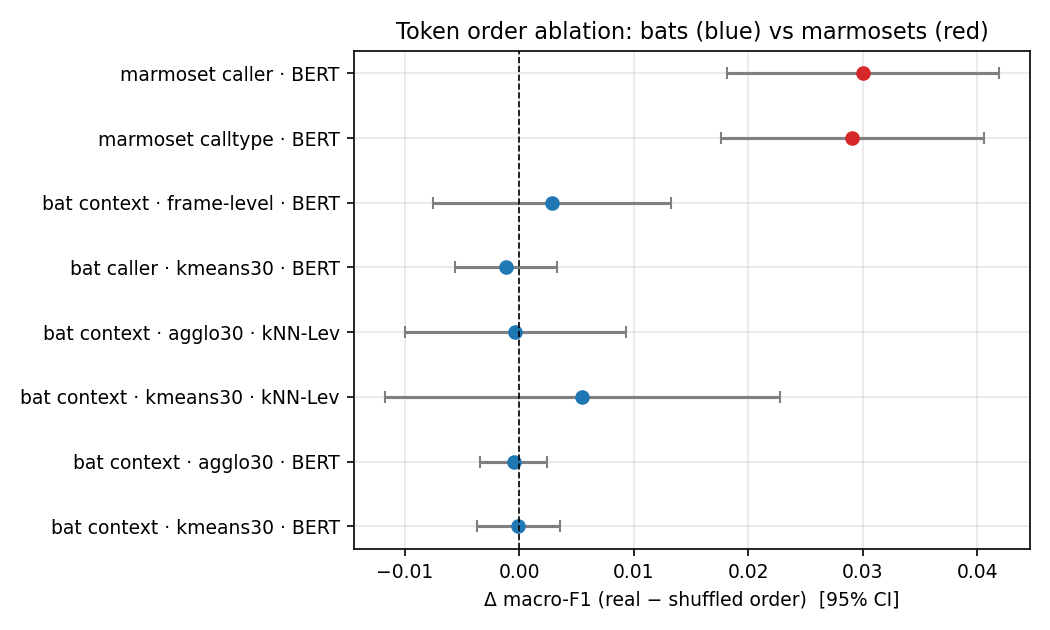
\includegraphics[width=\linewidth]{fig1_order_ablation.png}
\caption{Order ablation. Bats (blue) straddle 0 (n.s.); marmosets (red) significant but
small.}\label{fig:order}
\end{figure}

\textbf{Length is a confound.} Fig.~\ref{fig:length}: order is n.s.\ at short sequences
in both species; effects appear only at length, and at the matched 41--96 frame band
both species are n.s. We therefore report a small, length-modulated species contrast,
not a clean per-band dissociation.

\begin{figure}[t]\centering
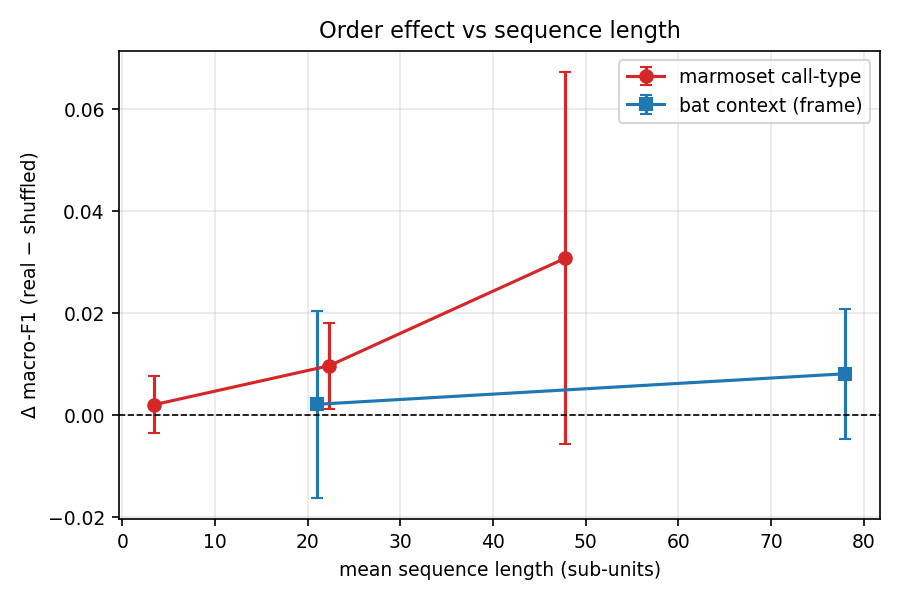
\includegraphics[width=\linewidth]{fig2_length_modulation.png}
\caption{Order effect vs.\ sequence length.}\label{fig:length}
\end{figure}

\textbf{Mechanism: sequential dependency, not diversity.} We refute a token-diversity
explanation (bats are \emph{more} diverse: 10.2 vs.\ 3.4 unique tokens/voc) and confirm
a sequential-dependency one (Fig.~\ref{fig:dep}): the previous token removes 77.5\% of
next-token uncertainty for marmosets vs.\ 13--33\% for bats; the bat's modest
frame-level dependency is context-irrelevant acoustic smoothness.

\begin{figure}[t]\centering
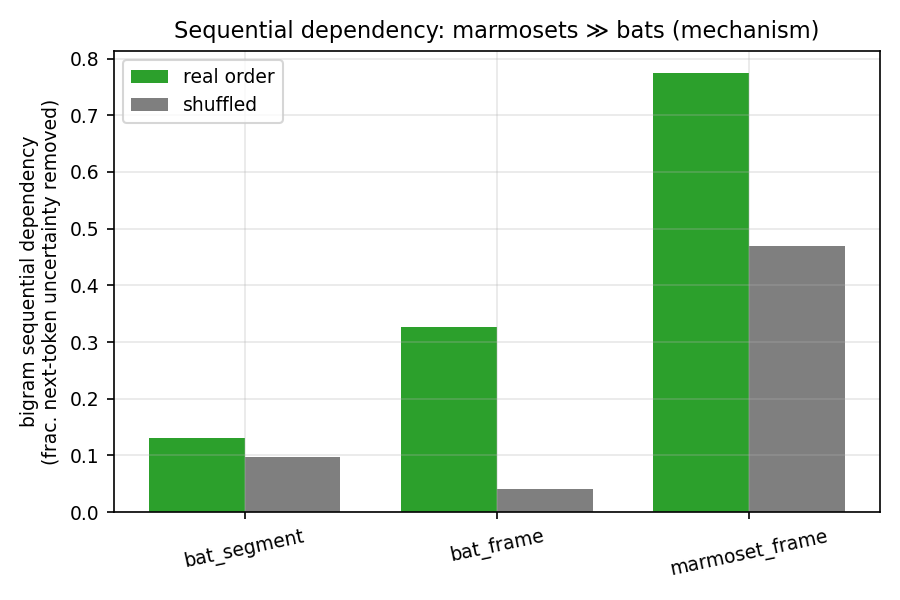
\includegraphics[width=\linewidth]{fig5_sequential_dependency.png}
\caption{Bigram sequential dependency: marmosets $\gg$ bats.}\label{fig:dep}
\end{figure}

\textbf{A domain-matched SSL tokenizer is the best discrete repertoire.}
Fig.~\ref{fig:ssl}: SSL $k$-means beats mel-UMAP at every $V$ (bat context macro-F1
0.34 vs.\ 0.28), surpassing a per-context DP-GMM density baseline (0.31); discretization
is near-lossless ($+0.025$ vs.\ continuous). SSL tokens also agree more with an
independent DTW acoustic reference \emph{despite lower silhouette} --- silhouette
mis-ranks quality.

\begin{figure}[t]\centering
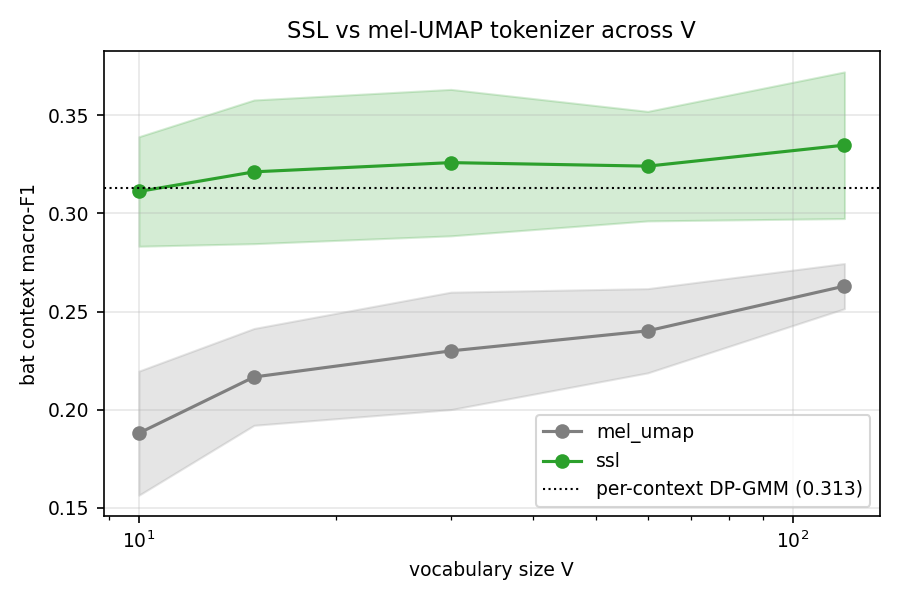
\includegraphics[width=\linewidth]{fig3_ssl_vocab.png}
\caption{SSL vs.\ mel-UMAP tokenizer across vocabulary size $V$.}\label{fig:ssl}
\end{figure}

\textbf{The SSL advantage is task-dependent --- and we show the cause.}
Fig.~\ref{fig:abl}: varying the contrastive positive-pair definition causally shifts
which task benefits. Same-vocalization positives maximize caller and destroy call-type;
same-frame augmentation recovers call-type and loses caller. The invariance selects the
served task; no SSL variant beats mel for fine within-call structure (call-type).

\begin{figure}[t]\centering
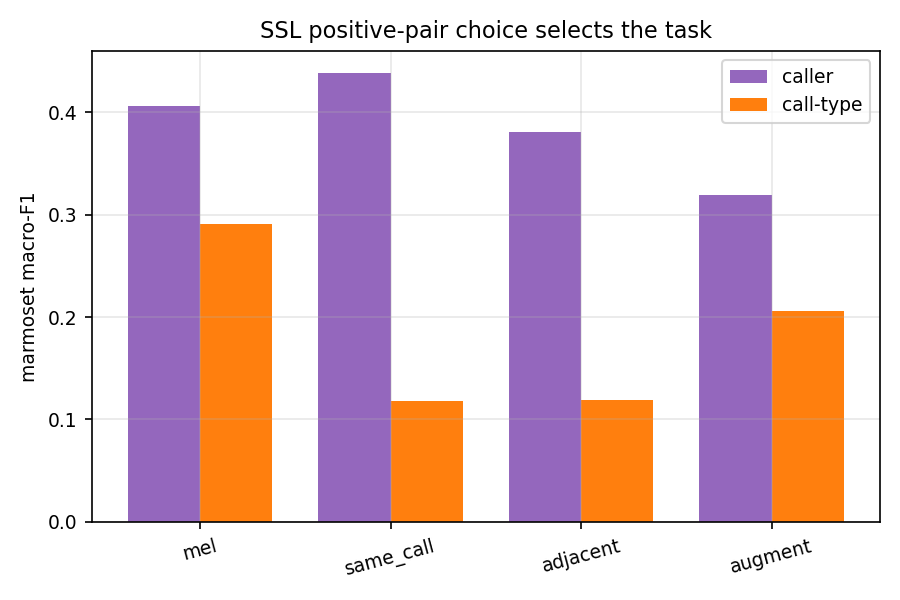
\includegraphics[width=\linewidth]{fig4_ssl_positive_ablation.png}
\caption{SSL positive-pair choice selects the downstream task.}\label{fig:abl}
\end{figure}

\textbf{Leakage caveat.} Per-context tokenization assigns disjoint token-ID ranges per
context; a token-sequence classifier reads the label off the range (bag-LR macro-F1
$\approx 1.0$). Per-context tokenizers must be evaluated by generative max-likelihood.

\section{Discussion}
Token-order effects in tokenized animal vocalizations are small and length-confounded;
the multiset dominates. ``Leverage sequential structure'' claims need shuffle, length,
and CI controls. A domain-matched SSL tokenizer is a strong, near-lossless discrete
representation whose bias is set by the contrastive invariance. \textbf{Limitations:}
small effect sizes limit per-band power; two species; analogous-but-not-identical
featurization; closed-set marmoset caller-ID.

\begin{thebibliography}{9}
\small
\bibitem{sarkar2025} E.~Sarkar and M.~Magimai-Doss. Towards Leveraging Sequential
Structure in Animal Vocalizations. arXiv:2511.10190, NeurIPS Workshop on AI for
Non-Human Animal Communication, 2025.
\bibitem{prat2017} Y.~Prat et al. Everyday bat vocalizations contain information about
emitter, addressee, context, and behavior. Sci.\ Rep., 2017.
\bibitem{sensorscan} M.~Golyadkin, V.~Pozdnyakov, L.~Zhukov, I.~Makarov. SensorSCAN:
Self-supervised learning and deep clustering for fault diagnosis. Artif.\ Intell., 2023.
\end{thebibliography}

\end{document}
